\documentclass[12pt]{article}
\usepackage[left=1cm, right=1cm, top=2cm,bottom=1.5cm]{geometry} 

\usepackage[parfill]{parskip}
\usepackage[utf8]{inputenc}
\usepackage[T2A]{fontenc}
\usepackage[russian]{babel}
\usepackage{enumitem}
\usepackage[normalem]{ulem}
\usepackage{amsfonts, amsmath, amsthm, amssymb, mathtools}

\usepackage{fancyhdr}
\pagestyle{fancy}
\renewcommand{\headrulewidth}{1.5pt}
\renewcommand{\footrulewidth}{1pt}

\usepackage{graphicx}
\usepackage[figurename=Рис.]{caption}
\usepackage{subcaption}
\usepackage{float}

%%Наименование папки откуда забирать изображения
\graphicspath{ {./images/} }

%%Изменение формата для ввода доказательства
\renewcommand{\proofname}{$\square$  \nopunct}
\renewcommand\qedsymbol{$\blacksquare$}

\addto\captionsrussian{%
	\renewcommand{\proofname}{$\square$ \nopunct}%
}
%% Римские цифры
\newcommand{\RN}[1]{%
	\textup{\uppercase\expandafter{\romannumeral#1}}%
}


\theoremstyle{definition}
\newtheorem{defn}{Опр:}
\newtheorem{rem}{Rm:}
\newtheorem{prop}{Утв.}
\newtheorem{exrc}{Упр.}
\newtheorem{lemma}{Лемма}
\newtheorem{theorem}{Теорема}
\newtheorem{corollary}{Следствие}

\newenvironment{cusdefn}[1]
{\renewcommand\thedefn{#1}\defn}
{\enddefn}



\DeclareRobustCommand{\divby}{%
	\mathrel{\text{\vbox{\baselineskip.65ex\lineskiplimit0pt\hbox{.}\hbox{.}\hbox{.}}}}%
}
\DeclareMathSymbol{\shortminus}{\mathbin}{AMSa}{"39}

\newcommand{\smallerrel}[1]{\mathrel{\mathpalette\smallerrelaux{#1}}}
\newcommand{\smallerrelaux}[2]{\raisebox{.1ex}{\scalebox{.75}{$#1#2$}}}

\newcommand{\smallin}{\smallerrel{\in}}
\newcommand{\smallnotin}{\smallerrel{\notin}}

\newcommand*{\medcap}{\mathbin{\scalebox{1.25}{\ensuremath{\cap}}}}%
\newcommand*{\medcup}{\mathbin{\scalebox{1.25}{\ensuremath{\cup}}}}%

\begin{document}
	\lhead{Математический анализ - I}
	\chead{Шапошников С.В.}
	\rhead{Лекция - 16}
\subsection*{Критерий Коши}

Пусть $f \colon D \to \mathbb{R}$, $a$ - предельная точка $D$.

\begin{theorem}
	Существует конечный предел функции $f(x)$: $\exists \, \lim\limits_{x\to a} f(x) \Leftrightarrow \forall \varepsilon > 0, \exists \, \delta > 0 \colon \forall x,y \in D$, \\ $0 < |x -a| < \delta \wedge 0 < |y - a| < \delta \Rightarrow |f(x) -f(y)| < \varepsilon$.
\end{theorem}

\begin{proof}\hfill\\
	$(\Rightarrow)$ Пусть $\lim\limits_{x \to a}f(x) =A$, по определению $\forall \varepsilon > 0, \, \exists \, \delta > 0 \colon \forall x \in D, \, 0 < |x-a| < \delta \Rightarrow |f(x) - A| < \varepsilon$. Пусть $ 0 < |x -a| < \delta \wedge 0 < |y - a| < \delta$, оценим разность $|f(x) - f(y)|$: $$|f(x) - f(y)| = |f(x) - A + A - f(y)| \leq |f(x) - A| + |f(y) - A| < 2 \varepsilon$$
	Таким образом, условие Коши проверено.
	
	$(\Leftarrow)$ Пусть $x_n \to a \wedge x_n \neq a$. Докажем, что $f(x_n)$ - сходится:\\
	$\forall \varepsilon > 0, \exists \, \delta > 0\colon \forall x,y \in D, \, 0 < |x -a| < \delta \wedge 0 < |y - a| < \delta \Rightarrow |f(x) -f(y)| < \varepsilon$. Поскольку $x_n \to a \Rightarrow$ \\
	$\Rightarrow \exists \, N \colon \forall n > N, \, 0<|x_n - a| < \delta$. Тогда по условию Коши, если взять $n, m > N \Rightarrow |f(x_n) - f(x_m)| < \varepsilon$. Следовательно, последовательность $f(x_n)$ сходится. 
	
	Проверим, что выбор $x_n$ не влияет на значение предела: \\
	Пусть $y_n \to a \wedge y_n \neq a$. Составим новую последовательность $z_n \colon x_1, y_1, x_2, y_2, \dotsc \Rightarrow z_n \to a \wedge z_n \neq a$. Доказали, что $f(z_n)$ - сходится, $f(x_n)$ и $f(y_n)$ - подпоследовательности. 
	
	Знаем, что пределы подпоследовательностей совпадают с пределом последовательности, если эта последовательность сходится $\Rightarrow \lim\limits_{x_n \to a}f(x_n) = \lim\limits_{y_n \to a}f(y_n)= \lim\limits_{z_n \to a}f(z_n) \Rightarrow$ предел не зависит от выбора $x_n$.
\end{proof}

\section*{Предел по базе}
Пусть $X \neq \varnothing$.

\begin{defn}
	\uwave{Базой} называется такой непустой набор $\mathfrak{B}$ подмножеств $X$, что 
	\begin{enumerate}[label={(\arabic*)}]
		\item $\varnothing \notin \mathfrak{B}$;
		\item $\forall U, V \in \mathfrak{B}, \, \exists \, W \in \mathfrak{B} \colon W \subset U \cap V$;
	\end{enumerate}
\end{defn}

\subsection*{Примеры}
\begin{enumerate}[label={\arabic*)}]
	\item Пусть $X = \mathbb{N}$, $\mathfrak{B} = \{\,\{n \colon n >N \} \,\}$. $\{n \colon n >N_1 \} \cap \{n \colon n >N_2 \} = \{n \colon n > \max{\{N_1, N_2 \}} \}$;
	
	\item Пусть $X = \mathbb{R}$, зафиксируем точку $a$, $\mathfrak{B} = \{(a - \delta, a + \delta)\setminus \{a\}, \, \delta >0  \} = \{ \mathcal{U}_\delta^\prime(a), \, \delta > 0 \}$ - проколотая окрестность точки $a$. $\mathcal{U}_{\delta_1}^\prime(a) \cap \mathcal{U}_{\delta_2}^\prime(a) = \mathcal{U}_{\min\{\delta_1, \delta_2\} }^\prime(a)$;
	
	\item Пусть $X = \mathbb{R}$, зафиксируем точку $a$, $\mathfrak{B} = \{(a - \delta, a + \delta), \, \delta >0 \}$ - легко проверяется, что это база;
	
	\item Пусть $X \neq \varnothing$, зафиксируем точку $a$, все множества содержащие $a$ - $\mathfrak{B} = \{B \colon a \in B \}$ - база.
\end{enumerate}

\begin{exrc}
	Доказать последний пример.
\end{exrc}
\newpage
Пусть $f \colon X \to \mathbb{R}$.

\begin{defn}
	Число $A$ называется \uwave{пределом} $f$ \uwave{по базе} $\mathfrak{B}$, если: 
	$$
		\forall \varepsilon > 0, \, \exists \, U \in \mathfrak{B} \colon \forall x \in U, \, |f(x) - A| < \varepsilon
	$$ 
	Обозначение $A = \lim\limits_{\mathfrak{B}}f$.
\end{defn}

\subsection*{Примеры}
\begin{enumerate}[label={\arabic*)}]
	\item $X = \mathbb{N}, \, f\colon \mathbb{N} \to \mathbb{R}, \, f(n) = a_n, \, \mathfrak{B} = \{\,\{n \colon n >N \} \,\}$. Тогда 
	$$\forall \varepsilon > 0, \exists \, \{n \colon n >N \} \Leftrightarrow \exists \, N \colon \forall n \in \{n \colon n >N \} \Leftrightarrow \forall n > N \Rightarrow |a_n - A| < \varepsilon$$
	Получили в точности определение предела последовательности.
	
	\item $X = \mathbb{R}, \, f\colon \mathbb{R} \to \mathbb{R}, \, \mathfrak{B} = \{ \mathcal{U}_\delta^\prime(a), \, \delta > 0  \}$. Тогда
	$$\forall \varepsilon > 0, \exists \, \mathcal{U}_\delta^\prime(a) \Leftrightarrow 0 < |x-a| < \delta \colon \forall x \in \mathcal{U}_\delta^\prime(a) \Rightarrow |f(x) - A| < \varepsilon$$
	Получили в точности определение предела функции по Коши.
\end{enumerate}

\begin{exrc}
	Что даст пример $3)$ и $4)$.
\end{exrc}

\begin{prop}
	Если $\lim\limits_{\mathfrak{B}}f = A \wedge \lim\limits_{\mathfrak{B}}f = B \Rightarrow A = B$.
\end{prop}
\begin{proof}
	$\forall \varepsilon > 0, \exists \, U \in \mathfrak{B} \colon \forall x \in U \Rightarrow |f(x) - A| < \varepsilon$ и $\forall \varepsilon > 0, \exists \, V \in \mathfrak{B} \colon \forall x \in V \Rightarrow |f(x) - B| < \varepsilon$. 
	По условию 
	$$\exists \, W \neq \varnothing \colon W \subset U \cap V \Rightarrow \forall x \in W \Rightarrow |A - B| \leq |A - f(x)| + |f(x) - B| < 2 \varepsilon$$ 
	Если $A \neq B$, то при $\varepsilon = \frac{A - B}{2}$ получаем противоречие: $|A-B| < |A -B|$.
\end{proof}

\begin{prop}
	Пусть $\lim\limits_{\mathfrak{B}}f = A \wedge \lim\limits_{\mathfrak{B}}g = B$. Тогда $\forall \alpha, \beta \in \mathbb{R}, \, \lim\limits_{\mathfrak{B}}(\alpha f + \beta g) = \alpha A + \beta B$.
\end{prop}

\begin{proof}
	$\forall \varepsilon > 0, \exists \, U \in \mathfrak{B} \colon \forall x \in U \Rightarrow |f(x) - A| < \varepsilon$ и $\exists \, V \in \mathfrak{B} \colon \forall x \in V \Rightarrow |g(x) - B| < \varepsilon$. 
	По свойству базы 
	$$\exists \, W \neq \varnothing \colon W \subset U \cap V \Rightarrow \forall x \in W \Rightarrow |\alpha f(x) + \beta g(x) - (\alpha A + \beta B)| \leq |\alpha| |f(x) - A| + |\beta| |g(x) - B| \leq (|\alpha| + |\beta|) \varepsilon $$
\end{proof}

\begin{prop}\textbf{(Монотонность)}:
	Пусть $\lim\limits_{\mathfrak{B}}f = A \wedge \lim\limits_{\mathfrak{B}}g = B$ и $\exists \, U \in \mathfrak{B} \colon \forall x \in U, \, f(x) \leq g(x) \Rightarrow A \leq B$.
\end{prop}

\begin{proof}
	$\forall \varepsilon > 0, \exists \, U_1 \in \mathfrak{B} \colon \forall x_1 \in U_1 \Rightarrow |f(x_1) - A| < \varepsilon \wedge  \exists \, U_2 \in \mathfrak{B} \colon \forall x_2 \in U_2 \Rightarrow |g(x_2) - A| < \varepsilon$. По свойству базы: $\exists \, W \subset U_1 \cap U_2 \cap U$ (для трех множеств можно получить утверждение циклически: найти элемент базы в пересечении двух множеств, затем пересечь этот элемент с третьим множеством). 
	$$\forall x \in W \Rightarrow A - \varepsilon < f(x) \leq g(x) < B + \varepsilon \Rightarrow A < B + 2\varepsilon$$
	Если $A > B$, то при $\varepsilon = \frac{A - B}{2} > 0$ мы получаем $A < B + 2\varepsilon = B + A - B \Rightarrow A < A \Rightarrow$ противоречие $\Rightarrow A < B$.
\end{proof}

\begin{exrc}
	Записать с помощью определения по базе предел: $\lim\limits_{x \to +\infty} f(x) = A$. Подсказка: рассмотреть в качестве элементов базы $\{x \colon x > a\}$ и выписать определение предела по базе.
\end{exrc}

\begin{exrc}
	Записать с помощью определения по базе предел: $\lim\limits_{x \to -\infty} f(x) = A$. 
\end{exrc}

\begin{exrc}
	Записать с помощью определения по базе предел: $\lim\limits_{x \to \infty} f(x) = A$. 
\end{exrc}

\newpage 
\section*{Непрерывность}

Пусть $f \colon D \to \mathbb{R}, \, a \in D$, то есть $f$ определена в точке $a$.

\begin{defn}
	Функция $f$ - \uwave{непрерывна в точке $a$ по множеству $D$}, если 
	$$\forall \varepsilon > 0, \exists \, \delta > 0 \colon \forall x \in D, \, |x-a| < \delta \Rightarrow |f(x) - f(a)| < \varepsilon$$
\end{defn}

Выбор множества $D$ имеет решающее значение, если например рассмотрим функцию Дирихле:
$$ 
	D(x) = 
	\begin{cases} 
		1, & x \in \mathbb{Q} \\
		0, & x \notin \mathbb{Q} 
	\end{cases}
$$
она не является непрерывной в $0$ (всюду разрывна). Но если рассматривать её на множестве рациональных чисел - это будет всюду непрерывная функция. Аналогично, на множестве иррациональных чисел.

\begin{rem}
	Если $a$ - изолированная точка $D$ (т.е. в некоторой окрестности, других точек кроме точки $a$ там нет) и $f$ - определена в $a$, то $f$ - непрерывна в точке $a$.  
\end{rem}

\begin{figure}[H]
	\centering
	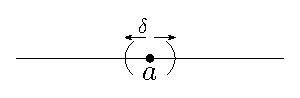
\includegraphics[width=0.2\textwidth]{16_1.eps}
	\caption{$a$ - изолированная точка.}
	\label{16_1}
\end{figure}

\textbf{Пример}: У функции в области определения могут быть изолированные точки $f(x) = \sqrt{x^2(x^2 - 1)}$. Она определена на множестве $(-\infty, -1) \cup \{0\} \cup (1, +\infty) \Rightarrow 0$ - изолированная точка.

\begin{figure}[H]
	\centering
	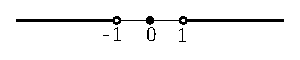
\includegraphics[width=0.3\textwidth]{16_2.eps}
	\caption{Область определения функции $f(x) = \sqrt{x^2(x^2 - 1)}$. $0$ - изолированная точка.}
	\label{16_2}
\end{figure}

В изолированной точке $a$ верно $|f(a) - f(a)| = 0 < \varepsilon$.

\begin{theorem}
	Следующие утверждения равносильны:
	\begin{enumerate}[label={(\arabic*)}]
		\item $f$ - непрерывна в точке $a$ множества $D$;
		\item $\forall x_n \in D, \, x_n \to a \Rightarrow f(x_n) \to f(a)$;
		\item $a$ - изолированная точка или $a$ - предельная точка $D$ и $\lim\limits_{x \to a} f(x) = f(a)$; 
	\end{enumerate}
\end{theorem}

\begin{proof}\hfill\\
	$(1) \Rightarrow (2)$: $\forall \varepsilon > 0, \exists \, \delta > 0 \colon \forall x \in D, \, |x-a| < \delta \Rightarrow |f(x) - f(a)| < \varepsilon$. Пусть $x_n \to a \Rightarrow$ по определению предела $\exists \, N \colon \forall n > N, \, |x_n - a|  < \delta \Rightarrow |f(x_n) - f(a)| < \varepsilon \Rightarrow f(x_n) \to f(a)$. 
	
	$(2) \Rightarrow (3)$: $a$ - изолированная точка $\Rightarrow$ ничего доказывать не нужно. Если $a$ - предельная точка, то надо показать, что $\lim\limits_{x \to a} f(x) = f(a)$: Распишем определение по Гейне $\Rightarrow \forall x_n \colon x_n \to a \wedge x_n \neq a \Rightarrow$\\ $f(x_n) \to f(a) \Rightarrow (2)$ - более общее, чем $(3) \Rightarrow$ верно.
	
	$(3) \Rightarrow (1)$: Если $a$ - изолированная точка, то $f$ - непрерывна в ней. Пусть $a$ - предельная точка, тогда по определению Коши: $\forall \varepsilon >0, \exists \, \delta > 0 \colon \forall x \in D, \, 0 < |x - a| < \delta \Rightarrow |f(x) - f(a)| < \varepsilon$. Хотим доказать, что  $\forall \varepsilon >0, \exists \, \delta > 0 \colon \forall x \in D, \, |x - a| < \delta \Rightarrow |f(x) - f(a)| < \varepsilon$. Если $x = a \Rightarrow |f(a) - f(a)| = 0 < \varepsilon$.
\end{proof}

\end{document}